\documentclass[a4paper,12pt]{article}
\usepackage[russian]{babel}
\usepackage[utf8]{inputenc}
\usepackage{amssymb}
\usepackage{graphicx}
\usepackage{listings}

\newtheorem{theorem}{Теорема}
\newtheorem{lemma}{Лемма}
\newtheorem{statement}{Утверждение}
\newtheorem{definition}{Опр.}

\newenvironment{proof}[1][Доказательство]{\begin{trivlist}
\item[\hskip \labelsep {\bfseries #1}]}{\end{trivlist}}

\newcommand{\qed}{\nobreak \ifvmode \relax \else
      \ifdim\lastskip<1.5em \hskip-\lastskip
      \hskip1.5em plus0em minus0.5em \fi \nobreak
      \vrule height0.75em width0.5em depth0.25em\fi}

\textwidth=17cm
\oddsidemargin=0mm

\begin{document}
\lstset{language=Java}

\section{Введение}

Цель данной работы – разработка программы, эмулирующей работу скрытого канала с мультипликативной помехой 
различного уровня интенсивности, использующей TRELLIS коды для помехоустойчивого кодирования передаваемой
информации. Варианты TRELLIS кодов выбираются из рекомендаций международного союза электросвязи 
ITU-T V.32 \cite{stV32}, V.32bis \cite{stV32bis}. 

\section{Постановка задачи}
Задача разбивается на несколько частей:

\begin{enumerate}
    \item Реализация алгоритма TRELLIS кодирования по рекоммендациям ITU-T V.32, V.32bis.
    \item Имитация канала связи с мультипликативной ошибкой.
    \item Реализация алгоритма декодирования Витерби.
\end{enumerate}

Заметим, что, поскольку разрабатываемое ПО носит исследовательский, а не прикладной характер, то разработка
велась исходя из необходимости обеспечить максимальное удобство при отладке, иногда даже в ущерб эффективности
в плане производительности.

\section{Описание алгоритмов}

\subsection{Алгоритм TRELLIS кодирования}
Алгоритм TRELLIS кодидования похож на алгоритмы сверточного кодирования тем, что кодирующее устройство может
находится в одном из нескольких состояний, в зависимости от которого происходит кодирование. Однако есть и
существенные отличия, главное состоит в том, что кодер выдает не цифровой, а аналоговый сигнал, таким образом
фазы кодирования и модуляции сигнала не разделяются.
Опишем данное утверждение более формально.

Кодом назовем функцию: $S \times \Sigma \rightarrow R^2 \times S$, где:
\begin{itemize}
	\item $S$ --- некоторое конечное множество состояний ($S_0 \ldots S_n$).
	\item $\Sigma$ --- алфавит, с которым работает кодер.
\end{itemize}
Данная функция по текущему состоянию $s \in S$ и текущему входоному символу $x \in \Sigma$ возвращает вектор
$\vec{a} \in R^2$ --- аналоговый сигнал (амплитуда и фаза), а также новое состояние.

Перейдем теперь к конкретным стандартам.

\subsubsection{V32}
Входной символ представляет собой четыре бита ($Q_1 \ldots Q_4$), т.е. $\Sigma = \{0, 1\}^4$. Кодер имеет $8$
состояний, т.е. три бита --- $S_0$, $S_1$, $S_2$. Схема вычисления функциий изображена на рисунке \ref{schemeV32}.

\begin{figure}
	\center{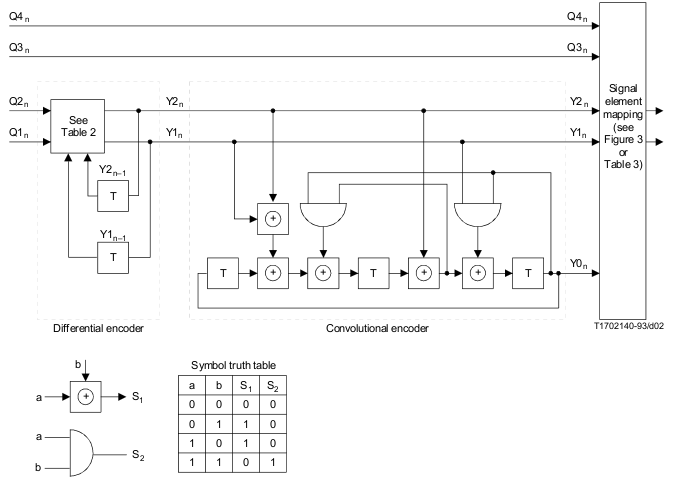
\includegraphics[scale=1]{pic/schemeV32.png}}
	\caption{Схема кодирующего устройства стандарта V32}
	\label{schemeV32}
\end{figure}

$Z^{-1}$ --- элемент задерживающий сигнал на один такт.
Под diffential encoder подсразумевается схема вычисляющая следующие форумулы:
\begin{itemize}
	\item $Y_{1n} = Q_{1n} \oplus Y_{1(n - 1)}$
	\item $Y_{2n} = (Q_{1n} \& Y_{1(n - 1)}) \oplus Y_{2(n - 1)} \oplus Q_{2n}$
\end{itemize}

Под element signal mapper подразумевается преобразователь сигнала в аналоговый вид. Преобразование осуществляется
при помощи схемы, изображееной на рисунке \ref{mapperV32}.

\begin{figure}
	\center{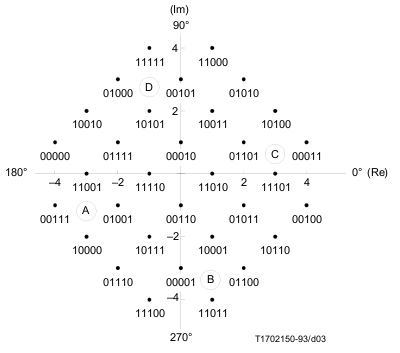
\includegraphics[scale=1]{pic/mapperV32.png}}
	\caption{Преобразователь сигнала стандарта V32}
	\label{mapperV32}
\end{figure}

\subsubsection{V32bis}
V32bis имеет небольшие отличия от V32. Входной символ представляет собой шесть бит, пятый и шетой биты передаются в 
signal mapper напрямую, остальные кодируются схемой указанной на рисунке \ref{schemeV32}. Signal mapper представлен
на рисунке \ref{mapperV32bis}

\begin{figure}
	\center{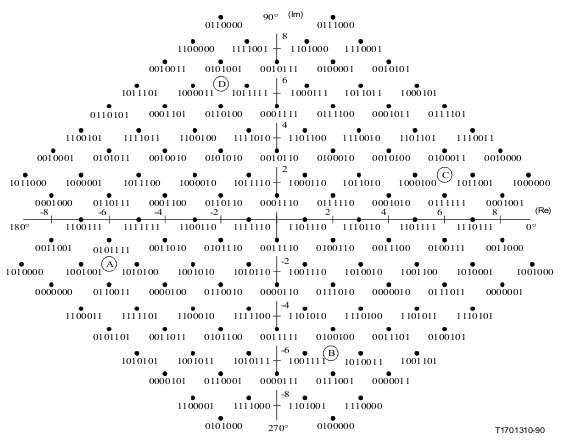
\includegraphics[scale=0.8]{pic/mapperV32bis.png}}
	\caption{Преобразователь сигнала стандарта V32bis}
	\label{mapperV32bis}
\end{figure}

\subsection{Имитация канала с ошибкой}
На закодированный (аналоговый) сигнал накладывается мультипликативная ошибка. 

Пусть $x = A e^{i\phi}$ --- закодированный сигнал, тогда $\vec{x'} = A\lambda e^{i\phi}$ --- сигнал в привнесенной
мультипликативной ошибкой, где $\lambda$ --- случайная величина с распределением: 
$\frac{1}{\sqrt{2\pi\sigma}}e^{-\frac{(\lambda - 1)^2}{2\sigma^2}}$

\subsection{Алгоритм Витерби для TRELLIS декодирования}
Алгоритм Витерби фактически основан на методе максимального правдоподобия.

Пусть мы хотим декодировать последовательность из $n$ символов. Алгоритм состоит из двух частей:
\begin{enumerate}
	\item Определение последовательности состояний кодера, передающего символы с наименьшей штрафной стоимостью
		(наиболее вероятную последовательность состояний).
	\item По последовательности состояний кодера определить переданные входные символы.
\end{enumerate}

Подробнее расммотрим каждый из этапов. На первом этапе алгоритм хранит промежуточные стоимости, $w_{ij}$ --- штрафная
стоимость достижения $j$-ого состояния после отправки $i$ символов.

При отработки очередного символа данные стоимости пересчитываются следующим образом:
$w_{(i + 1)j} = \min\limits_{k}(w_{ik} + cost(\vec{x_(i + 1)}, k, j))$

$cost(\vec{x_{i + 1}}, k, j) = \min\limits_{\{Q3, Q4, Y_{1i}, Y_{2i}, Q_1, Q_2\}}
(dist(\vec{x_{i + 1}}, E(Q_1, Q_2, Q_3, Q_4, k, Y_{1i}, Y_{2i})))$

$E$ --- кодер, минимум берется только по таким параметрам, которые дают состояние $j$. $dist$ --- евклидово расстояние
на плоскости.

По окончании первого этапа работы по значениям очевидно восстанавливается последовательность состояний, обеспечивающая
минимальную штрафную стоимость.

По последовательности и принятых символов очевидным образозов восстанавливается последовательность переданных символов
при помощи таблицы изображенной на рисунке \ref{decodeV32}.

\begin{figure}
	\center{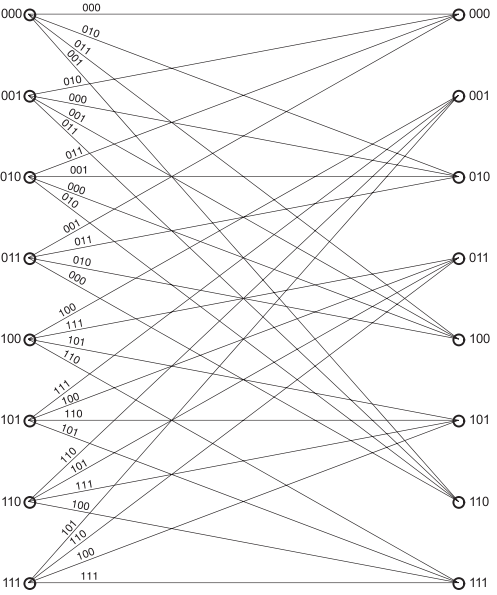
\includegraphics[scale=1]{pic/decodeV32.png}}
	\caption{Таблица декодирования по состояниям стандарта V32bis}
	\label{decodeV32}
\end{figure}

Вершины --- состояния, на ребраз изображены $Y_0, Y_1, Y_2$.

\section{Описание работы программы}
Программа написана на языке C++. Для ее компиляции необходимо иметь компилятор g++, а также библиотеку boost. Сборка
осуществляется при помощи утилиты make. Программа имеет консольный интерфейс. При запуске программе необходимо передать 
следующие параметры:
\begin{itemize}
	\item количество передаваемых битов;
	\item $\sigma$ --- параметр шума;
	\item версию стандарта --- V32, V32bis
\end{itemize}

Пример запуска программы под операционной системой linux: 

$./simulator ~~ 10000~~ 0.14 ~~ V32$

Выходным параметром является строка из символов: $\{*, _\}$, где $*$ --- ошибка декодирования, $_$ --- правильное
декодирование символа.

\section{Зaключение}
Таким образом, на данном этапе выполнения работы:
\begin{itemize}
	\item изучены алгоритм TRELLIS-кодирования и алгоритм декодирования Витерби;
	\item оба алгоритма реализованы в общем виде;
\end{itemize}

\bibliography{report}

\end{document}
